\chapter{恒定磁场}

\begin{introduction}
	
	\item \nameref{8.1}
	
	\item \nameref{8.2}
	
	\item \nameref{8.3}
	
	\item \nameref{8.4}
	
	\item \nameref{8.5}
	
	\item \nameref{8.6}
	
\end{introduction}

\section{磁场中的磁感应强度}\label{8.1}

$\bullet$ \textbf{磁场}

物质磁性的本质为电流. 无论是导线中的电流(传导电流)还是磁铁, 它们的本质都是电荷的运动, 而磁现象可以归结为运动的电荷之间的相互作用, 这种相互作用是通过磁场来传递的. 

\begin{figure}[H]
	\centering
	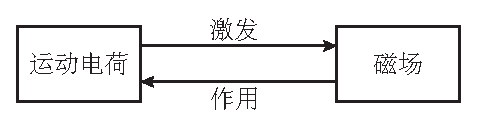
\includegraphics[scale=1.0]{C8-fig1.eps}
	\caption{磁场和运动电荷之间的关系}
\end{figure}

\begin{note}
	
	(1) 只有运动电荷才产生磁场, 静止电荷不产生磁场. 
	
	(2) 电场对静止电荷与运动电荷都有作用力, 而磁场仅对运动电荷有作用力. 
	
\end{note}


$\bullet$ \textbf{磁感应强度}

实验发现, 作用在运动电荷上的磁场力不仅与运动电荷的电荷有关, 还与运动电荷速度大小、方向有关. 

\begin{figure}[H]
	\centering
	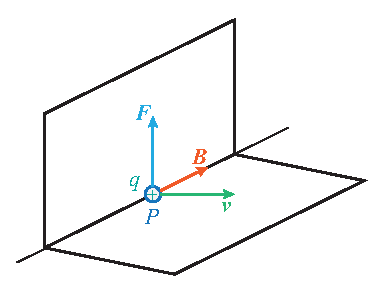
\includegraphics[scale=1.0]{C8-fig2.eps}
	\caption{运动电荷在磁场中受到力的作用}
\end{figure}

\begin{enumerate}[itemindent=1em]
	
	\item 对于点$P$, 若正电荷运动方向与该店磁场方向在同一直线上时, 磁场为0. 
	
	\item 当运动电荷以相同速率$v$沿不同方向过$P$点时, 电磁力总是既垂直于磁场方向, 有垂直于电荷运动方向, 即$\va*{F} \perp \va*{B}$, $\va*{F} \perp \va*{v}$. 
	
	\item 当运动电荷的速度垂直于磁场方向时, 此时受磁场力最大为$F_{\bot}$. 
	
\end{enumerate}

由于$F_{\bot}$与电荷$q$及其垂直于磁场方向速率$v_{\bot}$均成正比, 而$\dfrac{F_{\bot}}{qv_{\bot}}$在确定场点有确定的值, 且与$q$, $v_{\bot}$无关, 故定义磁感应强度

\begin{equation}
	B = \dfrac{F_{\bot}}{q v_{\bot}} \label{C8-eq1}
\end{equation}

国际单位制中, $B$的单位为$\textrm{N} \cdot \textrm{A}^{-1} \cdot \textrm{m}^{-1}$, 称为特斯拉, 用符号T表示. 

$\bullet$ \textbf{磁场叠加原理}

由若干运动电荷共同激发的磁场中, 某点的总的磁感应强度$B$等于各场源电荷激发的磁场在该点的磁感应强度的矢量和, 即

\begin{equation}
	B = \sum\limits_{i} B_i \label{C8-eq2}
\end{equation}

\section{毕奥—萨法尔定律}\label{8.2}

\begin{axiom}[毕奥—萨法尔定律]
	对于电流为$I$的线性电流, 取其上的长为$\dd{l}$的有向线元$\dd{\va*{l}}$, 规定$\dd{\va*{l}}$方向为线元处电流方向, $I\dd{\va*{l}}$称为电流元. $I\dd{\va*{l}}$在任一场点$P$处产生的磁感应强度为
	
	\begin{equation}
		\dd{\va*{B}} = \dfrac{\mu_0}{4 \pi} \dfrac{I \dd{\va*{l}} \times \va*{e_r}}{r^2} = \dfrac{\mu_0}{4 \pi} \dfrac{I \dd{\va*{l}} \times \va*{r}}{r^3} \label{C8-eq3}
	\end{equation}
	
	其中$\va*{r}$为电流元$I\dd{\va*{l}}$到场点$P$的经矢, 大小为$r$, 单位矢量为$\va*{e_r}$. 
	
	$\dd{\va*{B}}$大小为
	
	\begin{equation}
		\dd{B} = \dfrac{\mu_0}{4 \pi} \dfrac{I \dd{l} \sin \theta}{r^2} \label{C8-eq4}
	\end{equation}
	
	方向为$\dd{\va*{l} \times \va*{r}}$的方向, 垂直于$\dd{\va*{l}}$与$\va*{r}$决定的平面, 且满足右手定则. 
	
\end{axiom}

\begin{example}
	\textbf{一段载流直导线的磁场}
	
	\begin{figure}[H]
		\centering
		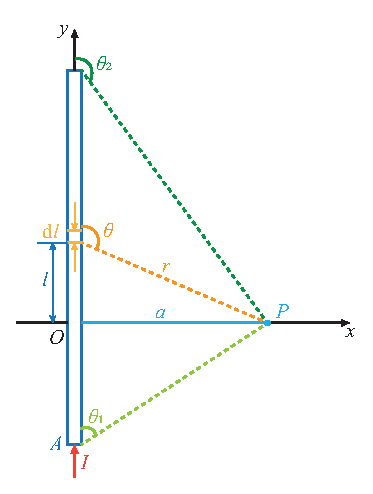
\includegraphics[scale=0.7]{C8-fig3.eps}
		\caption{一段载流直导线}
		\label{C8-fig3}
	\end{figure}
	
	\begin{solution}
		
		如图(\ref{C8-fig3})所示, $I\dd{l}$在$P$处产生的磁感应强度大小为
		
		\begin{equation*}
			\dd{B} = \dfrac{\mu_0}{4 \pi} \dfrac{I \dd{l} \cdot \sin \theta}{r^2}
		\end{equation*}
	
		积分得\footnote{注意$\theta_1$与$\theta_2$分别是指什么角. }
		
		\begin{equation*}
			B = \dfrac{\mu_0 I}{4 \pi a} \int_{\theta_1}^{\theta_2} \sin \theta \dd{\theta} = \dfrac{\mu_0 I}{4 \pi a} \qty(\cos \theta_1 - \cos \theta_2)
		\end{equation*}
		
		方向垂直纸面向里(由右手定则判断).
		
	\end{solution}
	
\end{example}

\begin{note}
	
	(1) 对于无限长直导线, 由上图知$\theta_1 \to 0$, $\theta_2 \to \pi$, 则
	
	\begin{equation*}
		B = \dfrac{\mu_0 I}{2 \pi a}
	\end{equation*}
	
	(2) 对于半无限长直导线, 假设一端延伸至无穷远(如上图B点), 则$\theta_2 = \pi$, 于是
	
	\begin{equation*}
		B = \dfrac{\mu_0 I}{4 \pi a} \qty(1 + \cos \theta) 
	\end{equation*}
		
	若$PA \perp$导线, 则$\theta_1 = \dfrac{\pi}{2}$, $\theta_2 = \pi$, 那么
	
	\begin{equation*}
		B = \dfrac{\mu_0 I}{4 \pi a}
	\end{equation*}
	
	(3) 对于直导线及其延长线上一点, $B = 0$.
	
\end{note}

\begin{example}
	\textbf{载流圆环轴线上的磁场} \quad 设有一半径为$R$的载流圆环, 通有电流$I$, 如图(\ref{C8-fig4})所示, 求过圆心垂直于圆平面的轴线上, 与圆心相距为$x$的$P$点的磁感应强度.
	
	\begin{figure}[H]
		\centering
		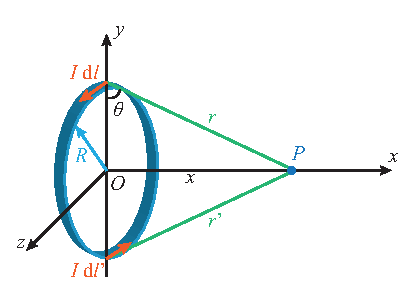
\includegraphics[scale=1.0]{C8-fig4.eps}
		\caption{载流圆环}
		\label{C8-fig4}
	\end{figure}
	 
	\begin{solution}
		
		\begin{equation*}
			B = \int \dfrac{\mu_0}{4 \pi} \dfrac{I \dd{l}}{r^2} \dfrac{R}{r} = \dfrac{\mu_0 I R^2}{2 \qty(R^2 + x^2)^{\frac{3}{2}}} 
		\end{equation*}
		
		方向沿$x$轴方向. 
		
		\begin{enumerate}[itemindent=1em]
			
			\item 当$x = 0$, 即圆心处的磁场
			
			\begin{equation*}
				B = \dfrac{\mu_0 I}{2 R}
			\end{equation*}
			
			\item 当$x \gg R$, 即轴线上无限远处的磁场为
			
			\begin{equation*}
				B = \dfrac{\mu_0 R^2 I}{2 x^3}
			\end{equation*}
			
		\end{enumerate}
		
	\end{solution}
	
\end{example}

\begin{example}
	\textbf{载流直螺线管轴线上的磁场} \quad 有一半径为$R$, 长为$l$的直螺线管, 单位长度上的线圈匝数为$n$, 当线圈中通有电流$I$时, 直螺线管内轴线上$P$点的磁感应强度. 
	
	\begin{figure}[H]
		\centering
		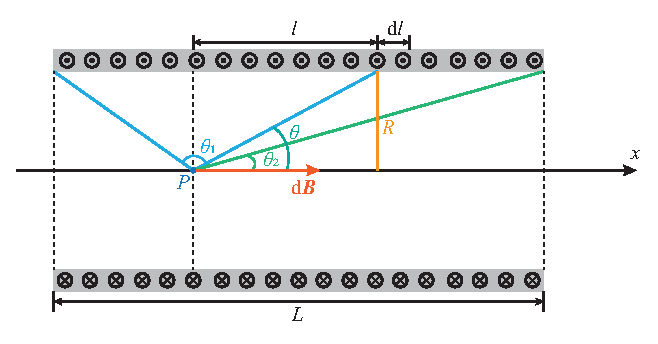
\includegraphics[scale=0.7]{C8-fig5.eps}
		\caption{载流直螺线管}
		\label{C8-fig5}
	\end{figure}
	
	\begin{solution}
		
		\begin{equation*}
			B = \int_{x_1}^{x_2} \dfrac{\mu_0 R^2 n I \dd{x}}{2 \qty(R^2 + x^2)^{\frac{3}{2}}} = \dfrac{\mu_0 n I}{2} \qty(\dfrac{x_2}{\sqrt{x_2^2 + R^2}} - \dfrac{x_1}{\sqrt{x_1^2 + R^2}}) = \dfrac{\mu_0 n I}{2} \qty(\cos \theta_2 - \cos \theta_1)
		\end{equation*}
		
		\begin{enumerate}[itemindent=1em]
			
			\item 当螺线管长度远大于半径时$(L \gg R)$, 螺线管可以认为是无限长, 此时$x_1 \to - \infty$, $x_2 \to + \infty$, 即$\theta_1 \to \pi$, $\theta_2 \to 0$, 于是
			
			\begin{equation*}
				B = \mu_0 n I
			\end{equation*}
			
			\item 对于长直密绕螺线管内任意一点的磁场, 有$B = \mu_0 n I$, 外部$B = 0$.
			
		\end{enumerate}
		
	\end{solution}

\end{example}

\begin{example}
	在真空中, 电流由长直导线1沿平行底边$ac$有向经$a$点流入一电阻均匀分布的正三角形框架, 再由$b$点沿$c$方向从三角框流出经长直导线2返回电源, 如图所示. 已知直导线电流为$I$, 三角形框的每一边长为$l$, 求正三角形中心点$O$处的磁感应强度. 
	
	\begin{figure}[H]
		\centering
		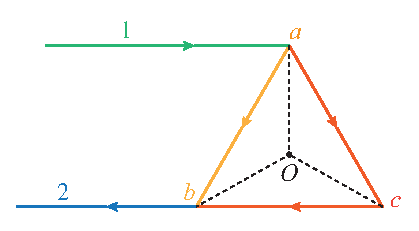
\includegraphics[scale=0.9]{C8-fig6.eps}
		\caption{正三角形框架}
		\label{C8-fig6}
	\end{figure}
	
	\begin{solution}
		
		由题意, 令$\va*{B}_1$, $\va*{B}_2$, $\va*{B}_{ab}$, $\va*{B}_{acb}$分别代表长直导线1, 2, 通电三角框$ab$和$ac$, $cb$边在$O$点产生的磁感应强度, 因此
		
		\begin{equation*}
			\va*{B} = \va*{B}_1 + \va*{B}_2 + \va*{B}_{ab} + \va*{B}_{acb}
		\end{equation*}
		
		(1) 对于$\va*{B}_1$: 
		
		对$O$点来说, 直导线1为半无限长通电导线, 有
		
		\begin{equation*}
			B_1 = \dfrac{\mu_0 I}{4 \pi \cdot \overline{Oa}}
		\end{equation*}
		
		方向垂直纸面向里. 
		
		(2) 对于$\va*{B}_2$: 
		
		由毕—萨定律, 有
		
		\begin{equation*}
			B_2 = \dfrac{\mu_0 I}{4 \pi \cdot \overline{Oe}} \qty[\cos \qty(\pi - \dfrac{\pi}{6}) - \cos \pi] = \dfrac{\mu_0 I}{4 \pi \cdot \overline{Oe}} \qty(1 - \dfrac{\sqrt{3}}{2})
		\end{equation*}
		
		方向垂直纸面向里. 
		
		(3) 对于$\va*{B}_ab$和$\va*{B}_acb$, 由于$ab$和$acb$并联, 则
		
		\begin{equation*}
			I_{ab} \cdot \overline{ab} = I_{acb} \cdot \qty(\overline{ac} + \overline{cb})
		\end{equation*}
		
		考虑到$ab = ac = cb$, 且$I_{ab} + I_{acb} = I$, 于是
		
		\begin{align*}
			I_{ab} &= \dfrac{2}{3} I \\
			I_{acb} &= \dfrac{1}{3} I
		\end{align*}
		
		由毕—萨定律, 得
		
		\begin{equation*}
			\va*{B} = \va*{B}_1 + \va*{B}_2
		\end{equation*}
		
		把$\overline{Oa} = \dfrac{\sqrt{3} l}{3}$, $\overline{Oe} = \dfrac{\sqrt{3} l}{6}$代入$\va*{B_1}$, $\va*{B_2}$得
		
		\begin{equation*}
			B = \dfrac{3 \mu_0 I}{4 \pi l} \qty(\sqrt{3} - 1)
		\end{equation*}
	
	    方向垂直于纸面向里. 
	
	\end{solution}
	
\end{example}

$\bullet$ \textbf{运动电荷的磁场}

对于$I\dd{\va*{l}}$的电流元, 若导线横截面为$S$, 载流子密度为$n$, 载流子电荷为$q$, 漂移速度为$\va*{v}$. 由电流定义

\begin{equation}
	I = \dv{Q}{t} = \dfrac{qnSv\dd{t}}{\dd{t}} = qnSv \label{C8-eq13}
\end{equation}

于是

\begin{align*}
	\dd{\va*{B}} &= \dfrac{\mu_0 I \dd{\va*{l}} \times \va*{e}_r}{4 \pi r^2} \\
	&= \dfrac{\mu_0}{4 \pi} \dfrac{qnS\dd{\va*{l}} \va*{v} \times \va*{e}_r}{r^2} \\
	&= \dfrac{\mu_0}{4 \pi} \dfrac{q\dd{N} \va*{v} \times \va*{e}_r}{r^2}
\end{align*}

$I\dd{\va*{l}}$方向与$\va*{v}$方向一致且$\dd{N} = nS\dd{l}$. 

故一个运动电荷$q$在点$P$产生磁场为

\begin{equation}
	B = \dv{\va*{B}}{N} = \dfrac{\mu_0}{4 \pi} \dfrac{q \va*{v} \times \va*{r}}{r^3} \label{C8-eq14}
\end{equation}

$\va*{B}$的方向垂直于$\va*{v}$和$\va*{r}$组成的平面且成右手系. 

若$q > 0$, $\va*{B}$与$\va*{v} \times \va*{r}$同向, 若$q < 0$, $\va*{B}$与$\va*{v} \times \va*{r}$反向. 

\begin{figure}[H]
	\centering
	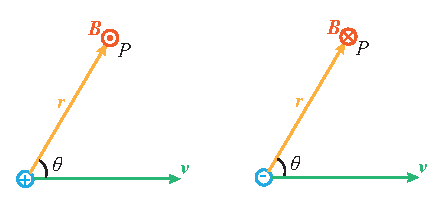
\includegraphics[scale=1.0]{C8-fig7.eps}
\end{figure}

\begin{equation*}
	B = \dfrac{\mu_0}{4 \pi} \dfrac{q v \sin\theta}{r^2}
\end{equation*}

\begin{example}
	在玻尔氢原子模型中, 电子绕核做匀速圆周运动, 已知电子速率为$v = 2.2 \times 10^6$ m/s, 轨道半径$r = 5.3 \times 10^{-11}$, 求电子运动在轨道中心产生的磁感应强度$\va*{B}$. 
	
	\begin{solution}
		
		电子在轨道中心产生的磁感应强度$\va*{B}$的大小为
		
		\begin{align*}
			B &= \dfrac{\mu_0}{4 \pi} \dfrac{e v \sin\qty(\dfrac{\pi}{2})}{r^2} \\ 
			&= \dfrac{\mu_0 e v}{4 \pi r^2} \\
			&= 10^{-7} \times \dfrac{1.6 \times 10^{-19} \times 2.2 \times 10^6}{\qty(5.3 \times 10^{-11})^2} \textrm{~T} \\
			&= 13 \textrm{~T}
		\end{align*}
		
		方向垂直纸面向里. 
		
	\end{solution}
	
\end{example}

\section{恒定磁场的性质}\label{8.3}

$\bullet$ \textbf{磁感应线}

\begin{enumerate}[itemindent=1em]
	
	\item 是无始无终涡旋状的闭合曲线, 或两端点伸向无穷远处. 
	
	\item 磁感应线和载流回路互相套合. 
	
	\item 任两条磁感应线不相交. 
	
\end{enumerate}

$\bullet$ \textbf{磁通量}

\begin{definition}[磁通量]
	
	磁场中通过某给定曲面的磁感应线的总条数称为通过该面的磁通量. 过面元$\dd{\va*{S}}$的磁通量为
	
	\begin{equation*}
		\dd{\varPhi} = B \cos \theta \dd{S} = \va*{B} \cdot \dd{\va*{S}}
	\end{equation*}
	
	其中, $\theta$为面元$\dd{\va*{S}}$的法线$\va*{e}_n$与$\va*{B}$之间的夹角. 
	
	故
	
	\begin{equation}
		\varPhi = \int_{S} \va*{B} \cdot \dd{S} \label{C8-eq5}
	\end{equation}
	
	若为封闭曲面则为
	
	\begin{equation}
		\varPhi = \oint_{S} \va*{B} \cdot \dd{S} \label{C8-eq6}
	\end{equation}
	
	国际单位制中, 磁通量的单位为韦伯(Wb), 且1 Wb = 1 T $\cdot$ m$^2$.
	
\end{definition}

$\bullet$ \textbf{磁场的高斯定理}

\begin{definition}[磁场的高斯定理]
	由于磁感应线是无头无尾的闭合曲线, 故进入和穿出任一闭合曲面S的磁感应线条数相等, 故闭合曲面总磁通量为零, 即
	
	\begin{equation}
		\oint_{S} \va*{B} \cdot \dd{S} = 0 \label{C8-eq7}
	\end{equation}

\end{definition}

磁场的高斯定理表明: \textbf{磁场为无源场, 磁感应线应为闭合曲线. }

$\bullet$ \textbf{磁场的安培环路定理}

\begin{definition}[磁场的安培环路定理]
	
	在恒定电流磁场中, 磁感应强度沿任一闭合路径上的线积分等于这个闭合路径L包围的所有电流代数和的$\mu_0$倍, 即
	
	\begin{equation}
		\oint_{L} \va*{B} \cdot \dd{l} = \mu_0 \sum\limits_{(内)} I_i \label{C8-eq8}
	\end{equation}
	
\end{definition}

磁场的安培环路定理表明: \textbf{磁场是非保守力场, 是有旋场, 称为涡旋场. }

\begin{example}	
	\textbf{载流长直导线} \quad 前面指出, 载流长直导线的磁感应线是一系列圆心在导线上的同心圆, 绕向与电流方向成右手螺旋关系, 且离电流$r$处$\va*{B}$的大小为
	
	\begin{equation*}
		B = \dfrac{\mu_0 I}{2 \pi r} 
	\end{equation*}
	
	可以证明: 
	
	\begin{enumerate}[itemindent=1em]
		
		\item 闭合路径未包含电流
		
		\begin{equation*}
			\oint_{L} \va*{B} \cdot \dd{l} = 0
		\end{equation*}
		
		\item 闭合路径包含电流$I$
		
		\begin{equation*}
			\oint_{L} \va*{B} \cdot \dd{l} = \mu_0 I
		\end{equation*}
		
		\item 空间中有$n$个电流, $k$个在闭合曲线内, $n - k$个在闭合曲线外
		
		\begin{equation*}
			\oint_{L} \va*{B} \cdot \dd{l} = \mu_0 \sum\limits_{i = 1}^{k} I_i
		\end{equation*}
		
		$I_i$在内部才算, 不在路径内部不算. 
		
	\end{enumerate}
	
\end{example}

\begin{example}
	\textbf{无限长均匀载流圆柱体内外的磁场}
	
	\begin{figure}[H]
		\centering
		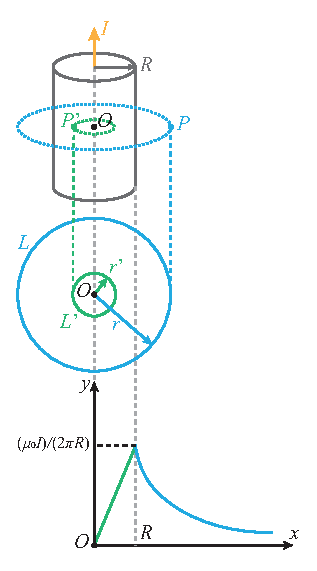
\includegraphics[scale=1.0]{C8-fig8.eps}
		\caption{无限长均匀载流圆柱体}
	\end{figure}
	
	\begin{solution}
		
		(1) 先计算圆柱体外$P$点($r > R$)的磁感应强度, 选择过$P$半径为$r$的圆周为积分回路$L$, 绕行方向和磁感线方向相同. 
		
		由安培环路定理得: 
	    
	    \begin{equation*}
	    	\oint_{L} \va*{B} \cdot \dd{l} = \mu_0 \sum\limits_{i} I_i
	    \end{equation*}
	    
	    在回路$L$上, 由于$B$大小处处相等, 且处处$\va*{B} \pll \dd{\va*{l}}$, 于是
	    
	    \begin{equation*}
	    	\oint_{L} \va*{B} \cdot \dd{l} = B \oint_{L} \dd{l} = 2 \pi r B
	    \end{equation*}
	    
		而$\sum\limits_{i} I_i = I$
		
		故
		
		\begin{equation*}
			2 \pi r B = \mu_0 I \Rightarrow B = \dfrac{mu_0 I}{2 \pi r}
		\end{equation*}
		
		(2) 再计算圆柱内($r < R$)的磁场, 取过圆柱体内部$P'$点的磁感应强度, 取过$P'$点半径为$r$的圆周为积分回路. 
		
		由于电流均匀分布, 则
		
		\begin{equation*}
			\sum\limits_{i} I_i = \dfrac{I \pi r^2}{\pi R^2} = 
			\dfrac{r^2}{R^2} I
		\end{equation*}
		
		由安培环路定理, 得
		
		\begin{equation*}
			\oint_{L} \va*{B} \cdot \dd{l} = 2 \pi r B = \mu_0 \dfrac{r^2}{R^2} I \Rightarrow B = \dfrac{\mu_0 I}{2 \pi} \dfrac{r}{R^2}
		\end{equation*}
		
		综上所述, 
		
		\begin{equation*}
			B = \begin{cases}
				\dfrac{\mu_0 I}{2 \pi} \dfrac{r}{R^2},~r \leq R \vspace{2ex} \\
				\dfrac{mu_0 I}{2 \pi r},~r > R
			\end{cases}
		\end{equation*}
		
		同理可得\textbf{载流圆柱面}的磁场
		
		\begin{equation*}
			B = \begin{cases}
				0,~r \leq R \\
				\dfrac{mu_0 I}{2 \pi r},~r > R
			\end{cases}
		\end{equation*}
		
	\end{solution}
	
\end{example}

\begin{example}
	\textbf{载流长直螺线管内的磁场} \quad 设一均匀密绕的空心长直螺线管, 单位长度有$n$匝线圈, 导线上通有电流$I$. 求其内部任一点$P$的磁感应强度. 
	
	\begin{figure}[H]
		\centering
		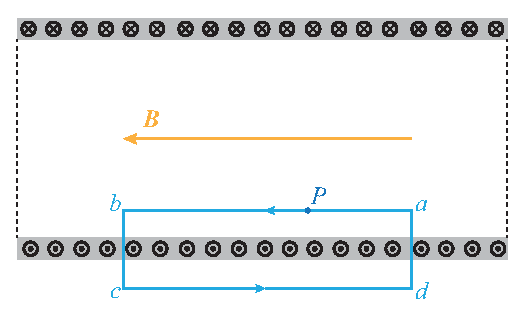
\includegraphics[scale=1.0]{C8-fig9.eps}
		\caption{载流直螺线管}
		\label{C8-fig9}
	\end{figure}
	
	\begin{solution}
		
		选择如图所示的环路, $\va*{B}$的环流为
		
		\begin{align*}
			\oint_{L} \va*{B} \cdot \dd{\va*{l}} &= \int_{a}^{b} \va*{B} \cdot \dd{\va*{l}} + \int_{b}^{c} \va*{B} \cdot \dd{\va*{l}} + \int_{c}^{d} \va*{B} \cdot \dd{\va*{l}} + \int_{d}^{a} \va*{B} \cdot \dd{\va*{l}} \\
			&= B \cdot \abs{ab} + 0 + 0 + 0 \\
			&= B \cdot \abs{ab}
		\end{align*}
		
		($B_{\text{外}} = 0$, 且管内部分$\va*{B} \perp \dd{\va*{l}}$).
		
		又$\sum\limits_{(内)} I = \abs{ab} \cdot n I$, 由安培环路定理可得
		
		\begin{equation*}
			B \cdot \abs{ab} = \mu_0 \cdot \abs{ab} \cdot n I \Rightarrow B = \mu_0 n I
		\end{equation*}
		
	\end{solution}
	
\end{example}

\begin{example}
	\textbf{载流螺绕环的磁场} \quad 设螺绕环内外半径分别为$R_1$, $R_2$, 环上均匀密绕$N$匝线圈, 线圈中通有电流$I$, 求螺绕环内部的磁感应强度
	
	\begin{figure}[H]
		\centering
		
\includegraphics[scale=1.0]{C8-fig10.eps}
		\caption{载流螺绕环}
	\end{figure}
	
	\begin{solution}
		
		螺绕环上的线圈绕得很紧密, 磁场几乎全部集中再螺绕环内. 取过点$P$且与螺绕环共心的圆周为积分回路$L$, 绕行方向为磁感应线方向. $L$上各点$B$相等, 处处$\va*{B} \pll \dd{\va*{l}}$, 于是
		
		\begin{equation*}
			\oint_{L} \va*{B} \cdot \dd{\va*{l}} = B \oint_{L} \dd{l} = 2 \pi r B
		\end{equation*}

		螺绕环内部电流走过$L$回路共$N$次, 则
		
		\begin{equation*}
			\sum\limits_{i} I_i = N I
		\end{equation*}
		
		根据安培环路定理, 有
		
		\begin{equation*}
			2 \pi r B = \mu_0 N I \Rightarrow B = \dfrac{\mu_0 N I}{2 \pi r} \quad (R_1 < r < R_2)
		\end{equation*}
		
		当螺线管很细, 孔径远小于平均半径$\overline{R} = (R_1 + R_2) / 2$时, 上式可写为
		
		\begin{equation*}
			B = \dfrac{\mu_0 N I}{2 \pi R}
		\end{equation*}
		
	\end{solution}
	
\end{example}

\begin{note}
	
	用安培环路定理求磁场分布很方便, 其一般步骤: 
	
	\begin{enumerate}[itemindent=1em]
		
		\item 从电流分布的对称性分析磁场分布的对称性;
		
		\item 选择合适的积分路径: 使$\oint_{L} \va*{B} \cdot \dd{\va*{l}}$中$\va*{B}$可以提出来, 一般而言, 在环路$L$上所求场点所在线段上$\va*{B}$大小相等, 方向与$\dd{\va*{l}}$平行, 在辅助线部分$\va*{B} = 0$, 或者$\va*{B} \perp \va*{l}$; 
		
		\item 由回路所围面积的电流代数和求$\sum\limits_{L\text{内}} I_i$; 
		
		\item 由安培环路定理$\oint_{L} \va*{B} \cdot \dd{\va*{l}} = \mu_0 \sum\limits_{L\text{内}} I_i$求出$\va*{B}$的大小, 并指出$\va*{B}$的方向.
		
	\end{enumerate}
	
\end{note}

\section{磁场对运动电荷的作用}\label{8.4}

$\bullet$ \textbf{洛伦兹力}

\begin{definition}[洛伦兹力]
	
	电荷量为$q$, 运动速度为$\va*{v}$的电荷在磁感应强度为$\va*{B}$的磁场中运动, 受到的洛伦兹力$\va*{F}$表示为
	
	\begin{equation}
		\va*{F} = q \va*{v} \times \va*{B} \label{C8-eq9}
	\end{equation}
	
	大小为
	
	\begin{equation*}
		F = qvB \cos\theta 
	\end{equation*}
	
	$\theta$为$\va*{v}$和$\va*{B}$的夹角. 
	
	\begin{figure}[H]
		\centering
		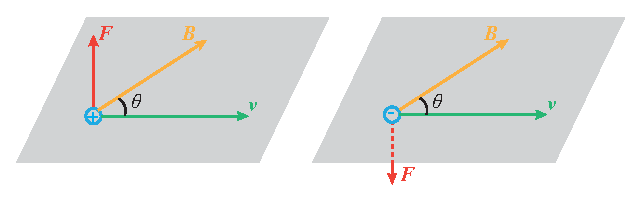
\includegraphics[scale=1.4]{C8-fig11.eps}
	\end{figure}
	
\end{definition}

\underline{洛伦兹力总与运动电荷方向垂直, 因此洛伦兹力对运动电荷不做功. }

\vskip 0.3cm

$\bullet$ \textbf{带电粒子在磁场中的运动}

在均匀磁场$\va*{B}$中, 当带电荷量为$q$, 质量为$m$的电子进入磁场中, 速度为$\va*{v}$, 则粒子受的洛伦兹力为$\va*{F} = q\va*{v}\va*{B}$. 

\begin{enumerate}[itemindent=1em]
	
	\item $\va*{v}{}\pll{}\va*{B}$, 则洛伦兹力$\va*{F}$粒子不受磁场影响. 
	
	\item $\va*{v} \perp \va*{B}$, 则$F = qvB$, 方向垂直于$\va*{v}$与$\va*{B}$组成平面, 指向$\va*{v} \times \va*{B}$方向. 
	
	特别地, 由牛顿第二定律
	
	\begin{equation}
		qvB = m \dfrac{v^2}{R} \label{C8-eq10}
	\end{equation}
	
	带电粒子做圆周运动的运动半径和周期
	
	\begin{align*}
		R &= \dfrac{mv}{qB} \\
		T &= \dfrac{2\pi R}{v} = \dfrac{2\pi m}{qB}
	\end{align*}
	
	\item $\left\langle \va*{v},\va*{B} \right\rangle = \theta$, 将$\va*{v}$分解为平行于$\va*{B}$的分量$\va*{v}_{\pll}$, 和垂直于$\va*{B}$的分量$\va*{v}_{\bot}$. 
	
	\begin{align*}
		\va*{v}_{\pll} &= v \cos\theta \\
		\va*{v}_{\bot} &= v \sin\theta \\
	\end{align*}
	
	则粒子在沿$\va*{B}$方向做匀速直线运动, 在垂直于$\va*{B}$的平面做匀速圆周运动. 
	
\end{enumerate}

$\bullet$ \textbf{霍尔效应}

以金属导体为例解释霍尔效应. 如图, 金属导体载流子为自由电子, 设载流子浓度为$n$, 自由电子漂移速率为$v$, 导体横截面积为$S$, 有

\begin{figure}[H]
	\centering
	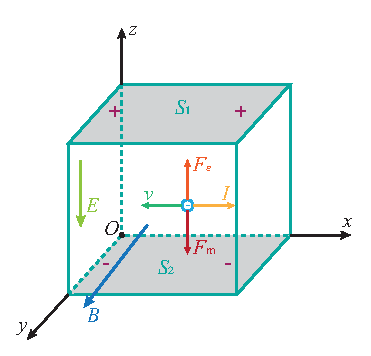
\includegraphics[scale=1.0]{C8-fig12.eps}
\end{figure}

\begin{equation}
	I = envS = envbd \Rightarrow v = \dfrac{I}{enbd} \label{C8-eq11}
\end{equation}

磁场中, 用左手判断得自由电子受到洛伦兹力向下, 大小为$F_{\textrm{m}} = evB$, 电子向下偏转. 下表面$S_2$带负电, 上表面$S_1$带正电, 于是上下表面出现电势差$U_{\textrm{H}}$.

当$U_{\textrm{H}}$满足

\begin{equation*}
	\begin{cases}
		eE = evB \\
		U_{\textrm{H}} = Eb
	\end{cases}
\end{equation*}

时, 有$U_{\textrm{H}} = Bbv$.

\vskip 0.3cm

又$v = \dfrac{I}{enbd}$, 则

\begin{equation}
	U_{\textrm{H}} = \dfrac{1}{en} \dfrac{BI}{d} = k\dfrac{BI}{d} \label{C8-eq12}
\end{equation}

其中, $k = \dfrac{1}{en}$为霍尔系数. 

\vskip 0.3cm

对于载流子不为电子而是正电荷的材料, 分析方法相同. 

\begin{example}
	如图所示, 一块半导体, 样品的体积为$a \times b \times c$, 沿$c$方向有电流, 沿厚度$a$边方向加有均匀外磁场$B$, 其均匀外磁场$\va*{B}$的方向和样品中电流方向垂直, 测得数据$a = 0.1$ cm, $b = 0.35$ cm, $c = 1$ cm, $I = 1.0$ mA, $B = 0.3$ T. 沿$b$边两侧的电势差$U = 665$ mV, 且上表面电势高. 问: 半导体为P型还是N型? 并求载流子浓度$n$.
	
	\begin{figure}[H]
		\centering
		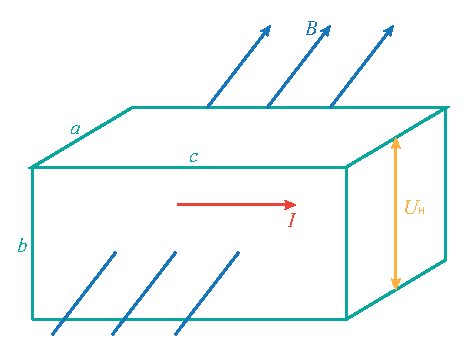
\includegraphics[scale=0.7]{C8-fig13.eps}
	\end{figure}
	
	\begin{solution}
		
		P型半导体为正电荷导电, N型半导体为负电荷导电. 
		
		由洛伦兹力, 
		
		(1) 若为负电荷导电, 则运动方向与$I$方向相反, 此时受向上的作用力, 电荷在上表面, 上表面带负电, 使得上表面电势较低, 与题意不符. 
		
		(2) 若为正电荷导电, 则运动方向与$I$相同, 此时受向上的作用力. 正电荷在上表面积累, 上表面电势更高. 
		
		所以这是P型半导体. 
		
		由霍尔效应知
		
		\begin{equation*}
			U_{\textrm{H}} = k \dfrac{IB}{a} = \dfrac{1}{qn} \dfrac{IB}{a}
		\end{equation*}
		
		代入题干数据和$q = e = 1.6 \times 10^{-19}$ C, 得
		
		\begin{equation*}
			n = \dfrac{IB}{q a U_{\textrm{H}}} = 2.82 \times 10^{20} \textrm{~m}^{-3}
		\end{equation*}
		
	\end{solution}
	
\end{example}

\section{磁场对电流的作用}\label{8.5}

$\bullet$ \textbf{安培定律}

\begin{axiom}[安培定律]
	
	真空磁场中, 有一根电流为$I$的导线, 在导线上任取一个电流元$I\dd{\va*{l}}$, 若导线横截面为$S$, 导线中自由电子数密度为$n$, 则$I\dd{\va*{l}}$内总电子数为$\dd{N} = nS\dd{l}$, 而每个自由电子所受洛伦兹力为$F = q\va*{v} \times \va*{B}$. 
	
	$I\dd{\va*{l}}$中所有电子受力为
	
	\begin{equation}
		\dd{\va*{F}} = nS\dd{l} \cdot q\va*{v} \times \va*{B} = nSqv \cdot \dd{\va*{l}} \times \va*{B} = I\dd{\va*{l}} \times \va*{B} \label{C8-eq15}
	\end{equation}
	
	这就是安培力, 其大小为$\dd{F} = I \dd{l} B \sin \alpha$, $\alpha$为$\dd\va*{l}$与$\va*{B}$的夹角, 方向与$\dd\va*{l} \times \va*{B}$方向一致. 
	
\end{axiom}

$\bullet$ \textbf{磁场对载流导线的作用}

求任意载流导线在磁场中受的作用力的步骤: 

\begin{enumerate}[itemindent=1em]
	
	\item 在载流导线上任取一个电流元$I\dd\va*{l}$;
	
	\item 根据安培定律写出电流元受安培力$\dd{\va*{F}} = I\dd{\va*{l}} \times \va*{B}$;
	
	\item 分析载流导线上各电流元所受的安培力方向是否相同, 如果方向相同, 须化适量积分为标量积分, 即
	
	\begin{equation*}
		F = \int_{L} \dd{F} = \int_{L} BI\sin\alpha \dd{l}
	\end{equation*}
	
	若方向不同, 则建立坐标系$Oxyz$, 写出$\dd{\va*{F}}$的分量式$\dd{\va*{F}_x}$, $\dd{\va*{F}_y}$, $\dd{\va*{F}_z}$, 再对这些分量进行积分, 即
	
	\begin{align*}
		F_x &= \int \dd{F_x} \\
		F_y &= \int \dd{F_y} \\
		F_z &= \int \dd{F_z}
	\end{align*}
	
	最后写成
	
	\begin{equation*}
		\va*{F} = F_x \va*{i} + F_y \va*{j} + F_z \va*{k}
	\end{equation*}
	
\end{enumerate}

\begin{note}
	
	(1) 若在均匀磁场中, 任意形状的载流导线在磁场中所受力的磁场力还可以进一步写成
	
	\begin{equation*}
		\va*{F} = \int_{L} I \dd{\va*{l}} \times \va*{B} = \int_{a}^{b} I \dd{\va*{l}} \times \va*{B} = I \qty(\int_{a}^{b} \dd{\va*{l}}) \times \va*{B} = I \va*{L} \times \va*{B}
	\end{equation*}
	
	\begin{figure}[H]
		\centering
		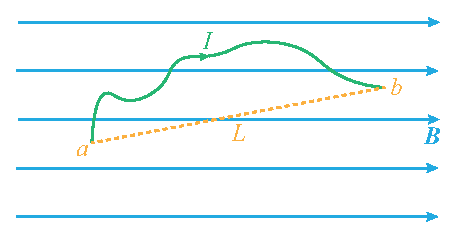
\includegraphics[scale=0.8]{C8-fig14.eps}
	\end{figure}
	
	其中$\va*{L}$表示从端点$a$指向端点$b$的有向线段, 即导线两端点间的位移矢量. 
	
	(2) 两长直导线电流方向相同的情况下, 受力为相互吸引力; 方向相反的情况下, 受力为相互排斥力.
	
	
\end{note}

\begin{example}
	载有电流$I_1$的长直导线和载有电流$I_2$的正方形框$ABCD$处在同一平面内, 电流方向如图所示, 正方形线框边长为$2a$, 它的中心到直导线的垂直距离为$b$, 求正方形线框每条边所受的力和线框所受合力. 
	
	\begin{figure}[H]
		\centering
		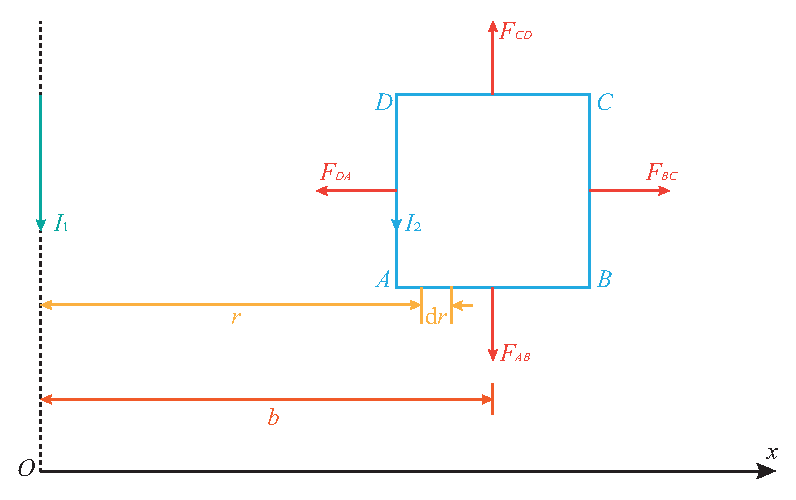
\includegraphics[scale=0.65]{C8-fig15.eps}
	\end{figure}
	
	\begin{solution}
		
		建立如图所示的一维坐标系.
		
		载流直导线电流$I_1$在线框所在空间产生的磁场为
		
		\begin{equation*}
			B_1 = \dfrac{\mu_0 I_1}{2 \pi r}
		\end{equation*}
		
		磁场方向垂直纸面向外, 由安培定律, 可得各边受力方向如图所示. 
		
		$DA$边各部分所在处的磁场时常量, 因此有
		
		\begin{equation*}
			F_{DA} = 2aI_2 B_1 = \dfrac{\mu_0 I_1 I_2 a}{\pi (b - a)}
		\end{equation*}
		
		同理, $BC$边受力为
		
		\begin{equation*}
			F_{BC} = \dfrac{\mu_0 I_1 I_2 a}{\pi (b + a)}
		\end{equation*}
		
		($AB$边受力的大小用积分法, 因为$AB$所处区域磁场不均匀)
		
		在$AB$上取距长直导线$r$处, 长为$\dd{r}$的电流元$I_2\dd{r}$受磁力为
		
		\begin{equation*}
			\dd{F} = I_2 \dd{r} B_1 \sin \dfrac{\pi}{2} = B_1 I_2 \dd{r}
		\end{equation*}
		
		在$AB$处, 每一个电流元所受磁力的方向一致, 均为垂直向下, 所以$AB$边受力的大小为
		
		\begin{equation*}
			F_{AB} = \int_{b-a}^{b+a} \dfrac{\mu_0 I_1}{2 \pi r} I_2 \dd{r} = \dfrac{\mu_0 I_1 I_2}{2 \pi} \ln \dfrac{b+a}{b-a}
		\end{equation*}
		
		同理, $CD$边受力大小为
		
		\begin{equation*}
			F_{CD} = \dfrac{\mu_0 I_1 I_2}{2 \pi} \ln \dfrac{b+a}{b-a}
		\end{equation*}
		
		$F_{AB}$和$F_{CD}$大小相等, 方向相反. 于是线框所受合力为
		
		\begin{equation*}
			F = F_{DA} - F_{BC} = \dfrac{\mu_0 I_1 I_2 a}{\pi} \qty(\dfrac{1}{b - a} - \dfrac{1}{b + a})
		\end{equation*}
		
		方向向左. 
		
	\end{solution}
	
\end{example}

$\bullet$ \textbf{磁场对载流线圈的作用}

\begin{definition}[载流线圈的磁矩]
	
	载流线圈的磁矩$\va*{m}$定义为
	
	\begin{equation}
		\va*{m} = NIS\va*{e}_n \label{C8-eq16}
	\end{equation}
	
	其中, $N$为线圈的匝数, $S$为线圈所围平面的面积, $I$为线圈中流过的电流, $\va*{e}_n$为线圈平面法线方向的单位矢量. 
	
	$\va*{e}_n$方向规定为: 当右手四指顺着电流方向回转时, 大拇指的指向就是载流线圈平面的法线方向. 
	
	磁矩$\va*{m}$的单位为A $\cdot$ m$^2$. 
	
\end{definition}

\begin{figure}[H]
	\centering
	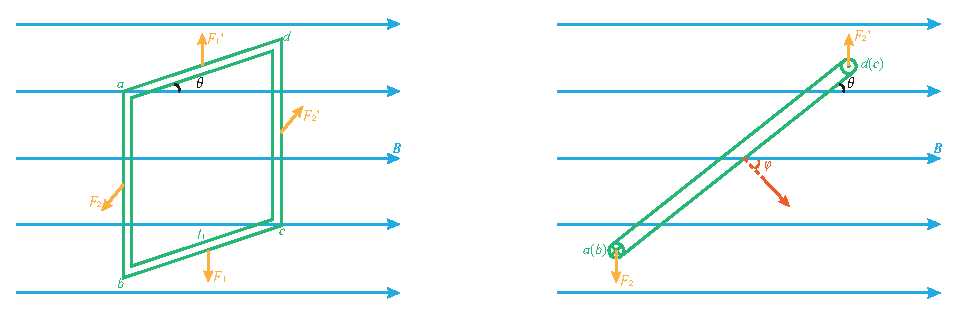
\includegraphics[scale=0.8]{C8-fig16.eps}
\end{figure}

导线$bc$和$ad$所受磁场力$F_1$和$F_1'$分别为

\begin{align*}	
	F_1 &= BIl_1 \sin\theta \\
	F_1' &= BIl_1 \sin\qty(\pi - \theta) = BIl_1 \sin\theta 
\end{align*}

两个力在同一直线上, 两个力大小相等而指向相反, 相互抵消. 

导线$ab$和$cd$所受的磁场作用力为

\begin{equation*}
	F_2 = F_2' = BIl_2
\end{equation*}

这两个力大小相等, 方向相反但不在同一直线上. 

$F_2$和$F_2'$形成一个力偶, 力臂为$l\cos\theta$, 所以磁场作用在线圈上的力矩

\begin{equation}
	M = 2F_2\cdot \dfrac{l_2}{2} \cos\theta = BIl_1l_2\cos\theta = BIS\cos\theta \label{C8-eq17}
\end{equation}

$S = l_1 l_2$为线圈的面积. 

若线圈有N匝, 那么线圈受力矩为

\begin{equation*}
	M = NBIS \sin\varphi
\end{equation*}

由于磁矩$\va*{m} = NIS\va*{e}_n$, 所以磁场作用在载流圈上的力矩

\begin{equation}
	\va*{M} = \va*{m} \times \va*{B} \label{C8-eq18}
\end{equation}

任意形状的平面线圈可以看成许多矩形线圈组合而成, 任意形状线圈在均匀磁场有

\begin{equation*}
	\begin{cases}
		\sum F = 0 \\
		\va*{M} = \va*{m} \times \va*{B}
	\end{cases}
\end{equation*}

\begin{example}
	一线圈由半径为$0.2$ m的$1/4$圆弧和相互垂直的两直线组成, 通以电流2 A, 把它放在磁感应强度为0.5 T的均匀磁场中, 磁感应强度$\va*{B}$的方向如图所示. 
	(1) 线圈平面与磁场垂直时, 圆弧$\wideparen{AB}$所受的磁力. 
	(2) 线圈平面与磁场成60$^{\circ}$角时, 线圈所受的磁力矩. 
	
	\begin{figure}[H]
		\centering
		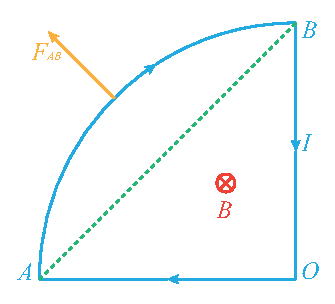
\includegraphics[scale=0.8]{C8-fig17.eps}
	\end{figure}
	
	\begin{solution}
		
		(1) 圆弧$\wideparen{AB}$所受的磁力 
		
		在均匀磁场中圆弧$\wideparen{AB}$通电, 圆弧所受的磁力与通有相同电流的$AB$直线所受的磁力相等, 则
		
		\begin{equation*}
			F = I \sqrt{2} R \cdot B = 2\sqrt{2} \times 0.2 \times 0.5 \textrm{~N} = 0.283 \textrm{~N}
		\end{equation*}
		
		方向与$AB$直线垂直, 与$OB$夹角为$45^{\circ}$.
		
		(2) 磁力矩为
		
		\begin{equation*}
			m = IS = \dfrac{\pi I R^2}{4}
		\end{equation*}
		
		\begin{figure}[H]
			\centering
			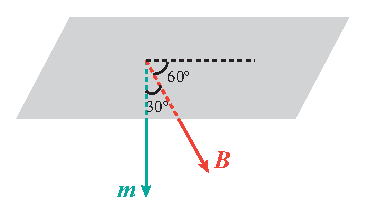
\includegraphics[scale=0.8]{C8-fig18.eps}
		\end{figure}
		
		线圈平面与$\va*{B}$成60$^{\circ}$角, 则$\va*{m}$与$\va*{B}$成30$^{\circ}$角. 
		
		故
		
		\begin{equation*}
			M = \abs{\va*{m} \times \va*{B}} = mB\sin 30^{\circ} = \dfrac{\pi I R^2}{4} B\sin 30^{\circ} = 1.57 \times 10^{-2} \textrm{~N} \cdot \textrm{m}
		\end{equation*}
		
		方向: 力矩$\va*{M}$将趋势线圈法线转向与$\va*{B}$平行. 
		
	\end{solution}
	
\end{example}

$\bullet$ \textbf{磁力的功}

\begin{enumerate}[itemindent=1em]
	
	\item 载流导线在磁场中运动时磁力的功
	
	\begin{figure}[H]
		\centering
		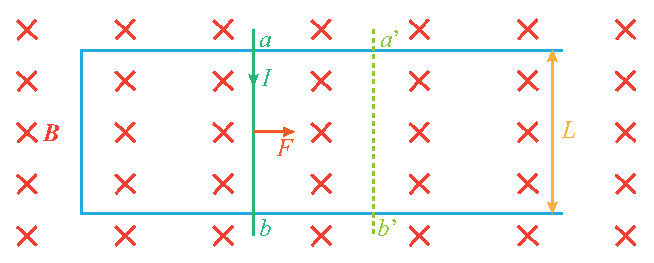
\includegraphics[scale=0.8]{C8-fig19.eps}
	\end{figure}
	
	当$ab$在磁场力的作用下向右移动到$a'b'$时, 磁力的功
	
	\begin{equation}
		A = F \cdot \abs{aa'} = BIl \abs{aa'} = BI\Delta S = I\Delta \phi \label{C8-eq19}
	\end{equation}
	
	即为电流乘回路包围面积内的磁通量的增量. 
	
	\item 载流线圈在磁场中转动时磁力矩的功
	
	$I$不变, 当线圈从$\theta_1$角转到$\theta_2$时, 磁力矩做的功
	
	\begin{equation}
		A = \int \dd{A} = I \int_{\theta_1}^{\theta_2} \dd{\phi} = I\qty(\phi_1 - \phi_2) = I \Delta \phi \label{C8-eq20}
	\end{equation}
	
	可以证明任意平面载流回路在均匀磁场中改变形状或位置时, 磁力或磁力矩做功都可以表示为
	
	\begin{equation}
		A = I \Delta \phi \label{C8-eq21}
	\end{equation}
	
	若$I$是随时间变化的, 则
	
	\begin{equation}
		A = \int I \dd{\phi} \label{C8-eq22}
	\end{equation}

\end{enumerate}

\begin{example}
	在均匀磁场中, 有一个通电流$I$, 半径为$R$的半圆形载流线圈, 如图所示, 线圈平面与磁场方向平行, 求: 
	(1) 线圈所受磁力对$y$轴的力矩;
	(2) 在这个磁力矩作用下线圈转过$\pi / 2$时, 磁力矩所做的功.
	
	\begin{figure}[H]
		\centering
		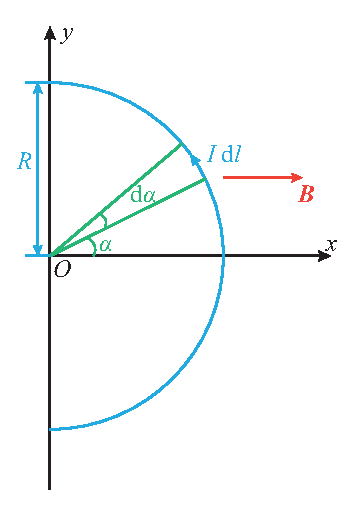
\includegraphics[scale=0.8]{C8-fig20.eps}
	\end{figure}
	
	\begin{solution}
		
		(1) 求解线圈对于$y$轴所受磁力矩有两种方法: 
		
		\textbf{方法一: 按力矩定义求}
		
		在半圆形线圈上取一个电流元$I\dd{l}$, 它所受到的磁力$\dd{F}$为
		
		\begin{equation*}
			\dd{F} = BI\dd{l} \cdot \sin\qty(\dfrac{\pi}{2} + \alpha) 
		\end{equation*}
		
		它对$y$轴的力矩
		
		\begin{equation*}
			\dd{M} = \dd{F} \cdot x = xBI\dd{l} \cdot \sin \qty(\dfrac{\pi}{2} + \alpha) 
		\end{equation*}
		
		这里有
		
		\begin{align*}
			x &= R \cos \alpha \\
			\dd{l} &= R \dd{\alpha}
		\end{align*}
		
		代入得
		
		\begin{equation*}
			\dd{M} = BIR^2 \cos^2 \alpha \dd{\alpha}
		\end{equation*}
		
		线圈对$y$轴所受磁力矩为
		
		\begin{equation*}
			M = \int_{-\frac{\pi}{2}}^{\frac{\pi}{2}} = BIR^2 \cos^2 \alpha \dd{\alpha} = \dfrac{\pi}{2} BIR^2
		\end{equation*}
		
		方向沿$y$轴正向, 故线圈将绕$y$轴沿逆时针方向转动. 
		
		\textbf{方法二: 直接用公式$\va*{M} = \va*{m} \times \va*{B}$计算}
		
		由于线圈磁矩$\va*{m}$大小为
		
		\begin{equation*}
			m = \dfrac{\pi}{2} R^2 I
		\end{equation*}
		
		$\va*{m}$的方向与$\va*{B}$的夹角为$\dfrac{\pi}{2}$, 磁力矩大小为
		
		\begin{equation*}
			M = m B \sin\dfrac{\pi}{2} = \dfrac{pi}{2} BIR^2
		\end{equation*}
		
		磁力矩的方向是$\va*{m} \times \va*{B}$的右螺旋方向, 即沿$y$轴的方向.
		
		(2) 磁力矩作用也可以用两种方法求解: 
		
		\textbf{方法一: 用定义求}
		
		若在磁力矩作用下线圈转过角度$\varphi$, 则$\va*{m}$与$\va*{B}$夹角为$\theta = \dfrac{\pi}{2} - \varphi$, 于是
		
		\begin{equation*}
			M = ISB \sin\theta = ISB\cos\varphi
		\end{equation*}
		
		当线圈转过$\dfrac{\pi}{2}$时, 磁力矩做的功为
		
		\begin{equation*}
			A = \int_{0}^{\frac{\pi}{2}} M \dd{\varphi} = \int_{0}^{\frac{\pi}{2}} ISB \cos\varphi \dd{\varphi} = ISB = \dfrac{\pi}{2} BIR^2
		\end{equation*}
		
		\textbf{方法二: 用$A = I \Delta \phi$求}
		
		\begin{equation*}
			A = I\Delta \phi = I \cdot \qty(\dfrac{\pi}{2} R^2 B - 0) = \dfrac{\pi}{2} BIR^2
		\end{equation*}
		
		可以看出, 用$\va*{M} = \va*{m} \times \va*{B}$及$A = I \Delta \phi$十分方便, 要注意磁力矩、磁矩均为矢量. 
		
	\end{solution}
	
\end{example}

\section{磁场中的磁介质}\label{8.6}

$\bullet$ \textbf{磁介质}

\begin{enumerate}[itemindent=1em]
	
	\item 放入磁场后能显示磁性, 产生附加磁场, 从而改变原来磁场分布的物质角做磁介质. 
	
	\item 磁介质中的磁感应强度$\va*{B}$应等于磁介质不存在时真空中的磁感应强度$\va*{B}_0$加上磁介质被磁化时激发的附加磁场的磁感应强度$\va*{B}'$, 即
	
	\begin{equation}
		\va*{B} = \va*{B}_0 + \va*{B}' \label{C8-eq23}
	\end{equation}
	
	\item 不同磁介质产生附加磁场$\va*{B}'$方向不同, 可以与$\va*{B}_0$相同, 也可相反. 
	
	\vskip 0.3cm
	
	\item 磁介质的相对磁导率$\mu_r = \dfrac{B}{B_0}$.
	
	\begin{table}[H]
		\centering
		\caption{磁介质的分类}
		\begin{tabular}{cl}
			\toprule[1pt]
			磁介质 & 相对磁导率 \\
			\hline
			抗磁质 & $\mu_r$的值略小于1(与原磁场方向相反) \\
			顺磁质 & $\mu_r$的值略大于1(与原磁场方向相同) \\
			铁磁质 & $\mu_r$的值远大于1, 且不为常量(与原磁场方向相同) \\
			\bottomrule[1pt]
		\end{tabular}
	\end{table}
	
	\item 磁化率: 定义为$\chi_{\textrm{m}} = \mu_r - 1$, 显然抗磁质的$\chi_{\textrm{m}} < 0$, 顺磁质的$\chi_{\textrm{m}} > 0$. 
	
	磁导率: 相对磁导率$\mu_r$和真空磁导率$\mu_0$的乘积. 
	
	\begin{equation}
		\mu = \mu_r \mu_0 \label{C8-eq24}
	\end{equation}

    $\mu$与$\mu_0$单位相同, 均为N/A$^2$.

\end{enumerate}

$\bullet$ \textbf{磁化强度与磁化电流}

类似于电介质中引入电极化强度$\va*{P}$的方法, 磁介质中引入一个宏观物理量, 磁化强度表示单位体积内分子磁矩的矢量和, 用$\va*{M}$表示. 

一般情况下, 各向同性磁介质中某点的磁化强度$\va*{M}$可以写成: 

\begin{equation}
	\va*{M} = \dfrac{\chi_{\textrm{m}}}{\mu} \va*{B} \label{C8-eq25}
\end{equation}

代入

\begin{align*}
	\chi_{\textrm{m}} &= \mu_r - 1 \\
	\mu &= \mu_0 \mu_r 
\end{align*}

得

\begin{equation}
	\va*{M} = \dfrac{1}{\mu_0} \qty(1 - \dfrac{1}{\mu_r}) \va*{B} \label{C8-eq26}
\end{equation}

$\bullet$ \textbf{磁介质中的安培环路定理}

\begin{definition}[磁介质中的安培环路定理]
	引入一个辅助物理量$\va*{H}$, 并令
	
	\begin{equation}
		\va*{H} = \dfrac{\va*{B}}{\mu_0} - \va*{M} = \dfrac{\va*{B}}{\mu} \label{C8-eq27}
	\end{equation}
	
	$\va*{H}$称为磁场强度, 单位是A/m. 
	
	进一步, 有
	
	\begin{equation}
		\oint_{L} \va*{H} \dd{l} = \sum\limits_{L\text{内}} I_0 \label{C8-eq28}
	\end{equation}
	
	这就是磁介质中的安培环路定理. 
	
	这表明: 磁场强度$\va*{H}$沿任意闭合曲线$L$的环流等于穿过以$L$为边界的任意曲面的传导电流的代数和. 
\end{definition}

实验发现: 磁化强度$\va*{M}$正比于介质中总的磁场强度$\va*{H}$, 关系为

\begin{equation}
	\va*{M} = \chi_{\textrm{m}} \va*{H} \label{C8-eq29}
\end{equation}

于是有

\begin{equation}
	\va*{B} = \mu_0 \qty(\va*{H} + \va*{M}) = \mu_0 \qty(1 + \chi_{\textrm{m}}) \va*{H} = \mu \va*{H} \label{C8-eq30}
\end{equation}

$\bullet$ 利用磁介质中的安培环路定理解题步骤: 

\begin{enumerate}[itemindent=1em]
	
	\item 分析电流分布和磁场分布的对称性, 在此基础上选取合适的闭合曲线L(环路L). 
	
	\vskip 0.3cm
	
	\item 利用$\displaystyle \oint_{L} \va*{H} \dd{\va*{l}} = \sum\limits_{L\text{内}} I_0$求出磁介质中磁场强度$\va*{H}$分布. 
	
	\item 利用$\va*{B} = \mu \va*{H}$, 求出$\va*{H}$分布. 
	
\end{enumerate}

$\bullet$ \textbf{铁磁材料}

\begin{figure}[H]
	\centering
	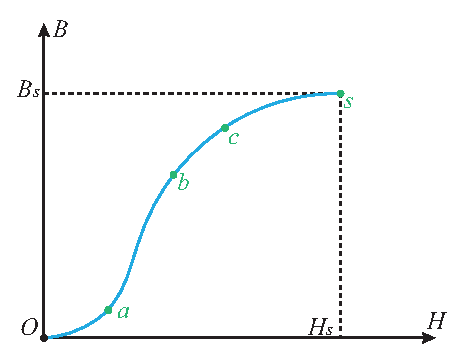
\includegraphics[scale=0.7]{C8-fig21.eps}
\end{figure}

图为铁磁质中$\va*{B}$与$\va*{H}$的关系曲线, $B_s$为饱和磁感应强度, $H_s$称为饱和磁场强度. 

当$H = 0$时, 铁磁质中仍可以有磁性, $B_{\textrm{R}}$称为剩磁, 当反向磁场$H$增加到$H_{\textrm{C}}$时$B$才等于0. 这种令铁磁质完全退磁时的磁场强度$H_{\textrm{C}}$称为矫顽力. 

\begin{table}[H]
	\centering
	\caption{铁磁材料分类}
	\begin{tabular}{cl}
		\toprule[1pt]
		铁磁材料 & 特点 \\
		\hline
		软磁类 & 磁导率大, 矫顽力小, 磁滞回线窄.  \\
		硬磁类 & 剩余磁感应强度$B_{\textrm{R}}$大, 矫顽力很大, 磁滞回线很宽 \\
		\bottomrule[1pt]
	\end{tabular}
\end{table}
